\pagenumbering{arabic}
%\documentclass[slides]{beamer}
\documentclass[mathserif]{beamer}
%\documentclass[slides,hyperref={pdfpagelabels=false}]{beamer}
%\documentclass[handout,gray]{beamer}
\usepackage[T1]{fontenc}
\usepackage[utf8]{inputenc}
\usepackage{textcomp}
\usepackage{verbatim}
\usepackage{amsbsy}
\usepackage{multicol}
\usepackage{booktabs} % Make some nice tables
\usepackage{ae,aecompl}

%%%%%%%%%%%% COULEURS %%%%%%%%%%%%%%%%%%%%%%%%%%%

\mode<presentation>
{
  \definecolor{beamerstructure}{RGB}{43,79,112}
  \definecolor{sidebackground}{RGB}{230,242,250}
  \definecolor{CTCC}{RGB}{133,188,228}
  \color{beamerstructure}
  \usetheme{default}
  \usepackage{courier}
  \beamertemplateballitem
\setbeamertemplate{navigation symbols}{}
%\setbeamertemplate{sidebar left}{\thispdfpagelabel{\insertframenumber}}
%\setbeamertemplate{footline}{\quad\insertframenumber}
%\usecolortheme{CTCC}
}
\usebackgroundtemplate{\includegraphics[width=1.02\paperwidth]{../templets/ctcc_general.jpg}}

\title{\\\vspace{1cm}
Low-scaling Hartree-Fock theory \\
using multiwavelets}
%\subtitle{\textcolor{magenta}{My subtitle (if applicable)}}
\author{Stig Rune Jensen}
\institute[CTCC]{\\[-6mm]stig.r.jensen@uit.no\\[6mm]University of Troms\o\\[6mm]
\includegraphics[height=1.5cm]{../templets/uio.pdf}\hspace{1cm} 
\includegraphics[height=1.5cm]{../templets/sff.pdf}\hspace{1cm}
\includegraphics[height=1.5cm]{../templets/uit.pdf}}
\date{Gran, \today}

\newcommand{\gb}[1]{green!#1!black}
\newcommand{\rb}[1]{red!#1!black}
\newcommand{\bb}[1]{blue!#1!black}
\newcommand{\coleq}{red!60!black}
\newcommand{\du}{\textrm{d}}

\usepackage{multicol}
\newcommand{\mydef}{\stackrel{\text{def}}{\hbox{=}}} 

\begin{document}

\footnotesize
\setlength{\unitlength}{\textwidth}

{
\usebackgroundtemplate{\includegraphics[width=1.02\paperwidth]{../templets/ctcc_forside.jpg}}
\maketitle
}

\begin{frame}
    \frametitle{Why low-scaling?}
	\begin{center}
	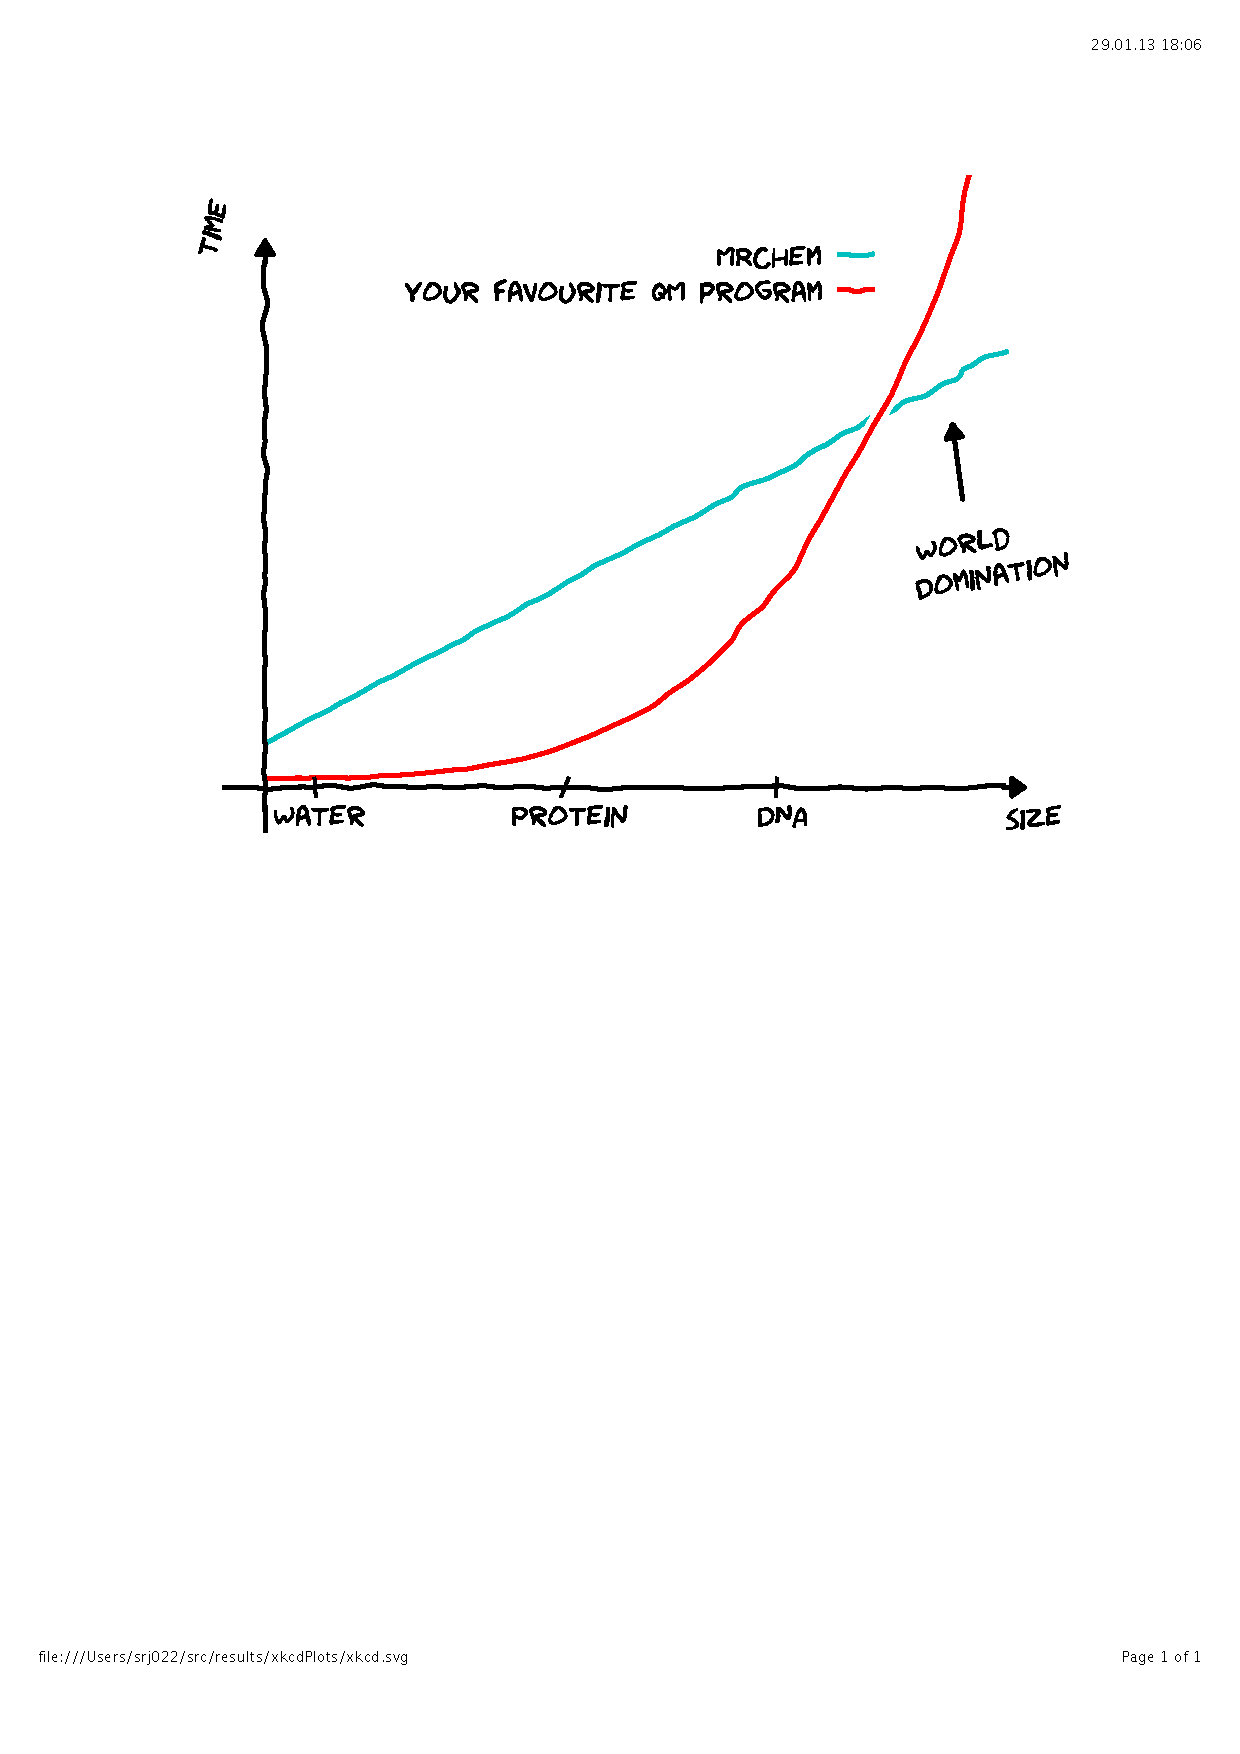
\includegraphics[bb = 80 430 530 750, clip, scale=0.5]{figures/xkcd.pdf}
	\end{center}
\end{frame}

\begin{frame}
    \frametitle{Outlook}
    \begin{itemize}
	\item The multiwavelet basis
	\ \\
	\ \\
	\item Hartree-Fock theory in the MW basis
	\ \\
	\ \\
	\item Localization of orbitals
	\ \\
	\ \\
	\item Results
    \end{itemize}
    \ \\
    \ \\
\end{frame}

\begin{frame}
    \frametitle{Functions in the MW basis}
    \ \\
    \ \\
    \begin{columns}
    \begin{column}{.48\textwidth}
	\begin{itemize}
	    \item Polynomial basis
	    \item 3D space divided in cubic cells
	\end{itemize}
    \end{column}%
    \hfill%
    \begin{column}{.48\textwidth}
	\begin{itemize}
	    \item Adaptive resolution
	    \item Guaranteed precision
	\end{itemize}
    \end{column}%
    \end{columns}
    \ \\
    \ \\
    \begin{center}
    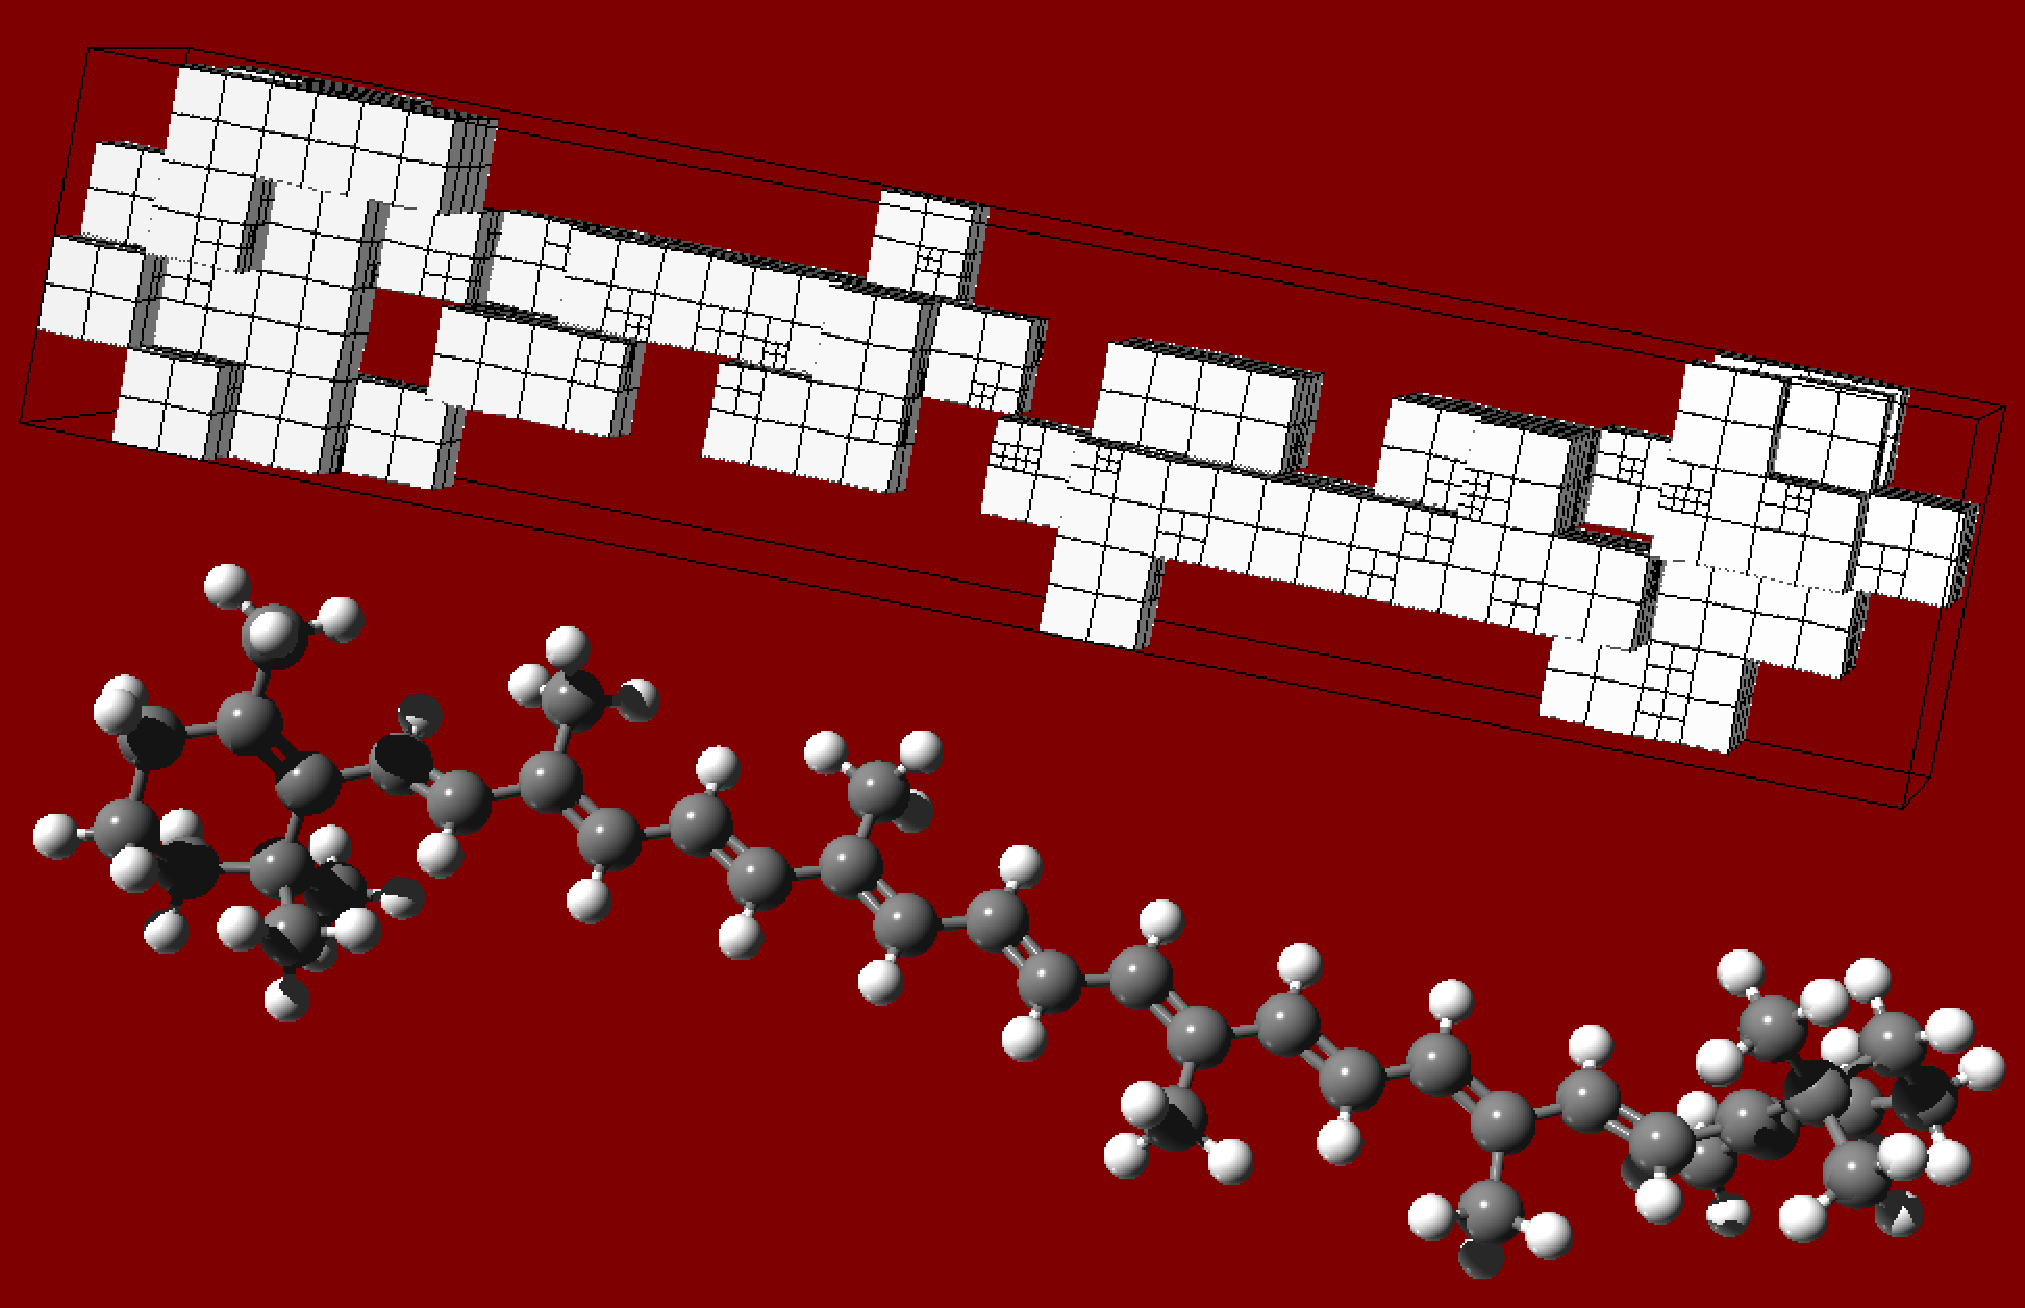
\includegraphics[scale=0.2]{figures/adapGrid.pdf}
    \end{center}
\end{frame}

\begin{frame}
    \frametitle{Operators in the MW basis}
    MW basis well suited for applying integral operators
    \begin{equation}
	\nonumber
	g(\boldsymbol{r}) = \int K(\boldsymbol{r} - \boldsymbol{r'}) 
	    f(\boldsymbol{r'}) d\boldsymbol{r'}
    \end{equation}
    which have been highly optimized and parallelized, and are linear scaling
    \ \\
    \ \\
    \pause
    \begin{columns}
    \begin{column}{.48\textwidth}
    \ \\
    \ \\
    \begin{itemize}
	\item Poisson kernel (electrostatics \\
	    and Hartree-Fock exchange) \\
	    \ \\
	\item Bound State Helmholtz (BSH) \\
	    kernel (Hartree-Fock equations) \\
	    \ \\
    \end{itemize}
    \end{column}
    \begin{column}{.48\textwidth}
    \ \\
    \begin{equation}
	\nonumber
	P(\boldsymbol{r}-\boldsymbol{r}') = 
	    \frac{1}{4\pi}\ \frac{1}{|\boldsymbol{r}-\boldsymbol{r}'|}
    \end{equation}
    \ \\
    \ \\
    \begin{equation}
	\nonumber
	H^{\epsilon}(\boldsymbol{r}-\boldsymbol{r}') = \frac{1}{4\pi}\ 
	    \frac{e^{-\sqrt{-2\epsilon} |\boldsymbol{r}-\boldsymbol{r}'|}}{|\boldsymbol{r}-\boldsymbol{r}'|}
    \end{equation}
    \end{column}
    \end{columns}
\end{frame}

\begin{frame}
    \frametitle{Hartree-Fock theory in the MW basis}
    Hartree-Fock equations for orbitals $\phi_i$ with energy $\epsilon_i$
    \begin{align}
	\nonumber
	\Big[-\frac{1}{2}\nabla^2 + V_{eff}(\boldsymbol{r}) + \hat{K}\Big]
	\phi_i(\boldsymbol{r}) =&\ \epsilon_i \phi(\boldsymbol{r})\\
	\nonumber
	\ & \ \\
	\nonumber
	\Big[-\nabla^2 - 2\epsilon_i\Big]\phi_i(\boldsymbol{r}) =&\ 
	    -2\ \Big(V_{eff}(\boldsymbol{r})+\hat{K}\Big)\phi_i(\boldsymbol{r})\\
	\nonumber
	\phi_i(\boldsymbol{r}) =&\ -2\int H^{\epsilon_i}(\boldsymbol{r}-\boldsymbol{r}')\
	    \Big[\Big(V_{eff}(\boldsymbol{r}') + \hat{K}\Big) 
	    \phi_i(\boldsymbol{r}')\Big] d\boldsymbol{r}'
    \end{align}
    \ \\
    \ \\
    using the BSH Green's kernel.\\
    \ \\
    \pause
    Solved self-consistently by straightforward iteration\\
    \begin{equation}
        \nonumber
        \phi^{n+1}_i(\boldsymbol{r}) =\ 
	    -2\int H^{\epsilon^n_i}(\boldsymbol{r}-\boldsymbol{r}')\ \Big[\Big(V^n_{eff}
	    (\boldsymbol{r}') + \hat{K}\Big) \phi^n_i(\boldsymbol{r}')\Big] 
	    d\boldsymbol{r}'
    \end{equation}
    \ \\
    \ \\
    \tiny \it{M. H. Kalos; "Monte Carlo calculations of the ground state of three- and 
	    four-body nuclei", Physical Review (1962)}
\end{frame}

\begin{frame}
    \frametitle{Coulomb potential}
    The Coulomb potential is given by the Poisson operator
    \begin{equation}
	\nonumber
	V_{coul}(\boldsymbol{r}) = 
	    \int P(\boldsymbol{r} - \boldsymbol{r}') \Big[ \rho(\boldsymbol{r}')\Big] 
	    d\boldsymbol{r}'
    \end{equation}
    \ \\
    \ \\
    \pause
    Coulomb potential of diamond clusters $C_{(2n+3)(n+2)(n+1)/6}H_{2(n+2)(n+1)}$
    \begin{center}
    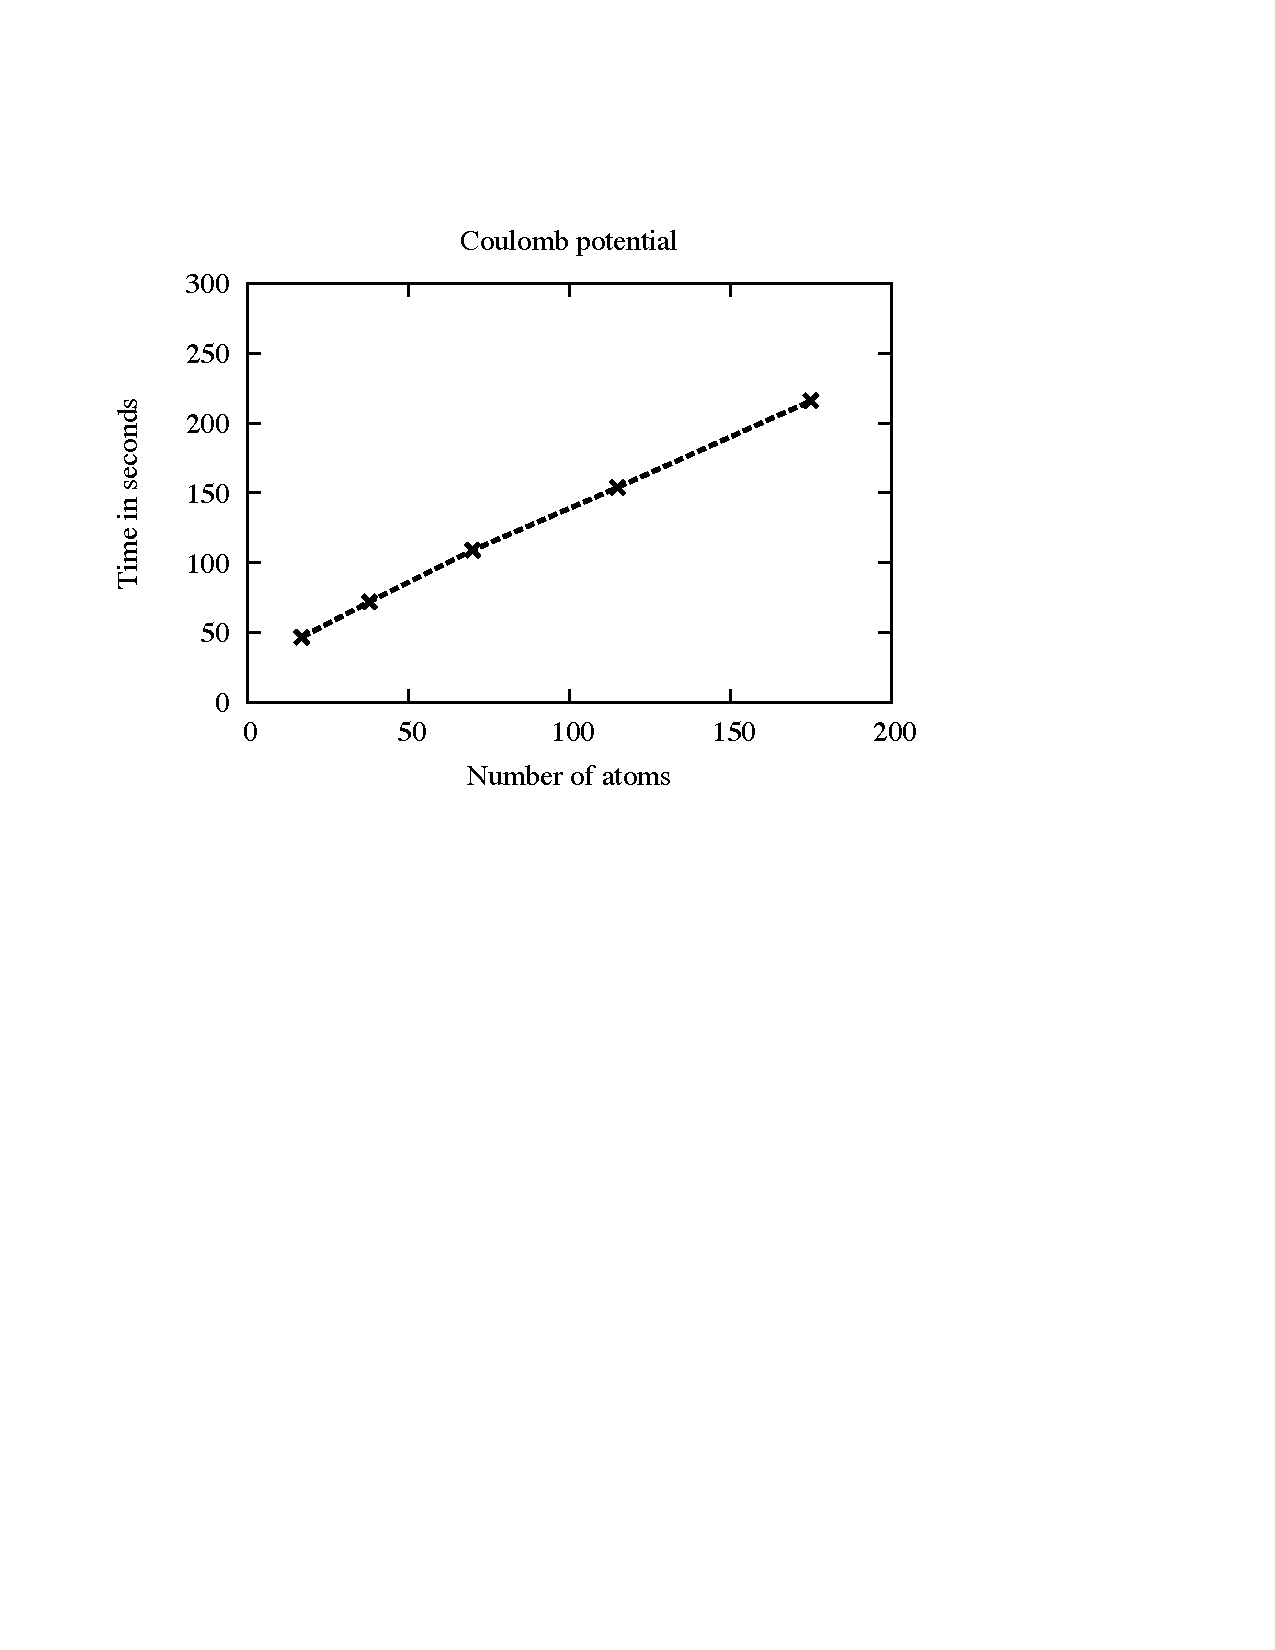
\includegraphics[bb = 50 400 500 690, clip, scale=0.5]{figures/coulombScaling.pdf}
    \end{center}
\end{frame}

\begin{frame}
    \frametitle{Hartree-Fock exchange}
    The Exchange operator can be decomposed into a sum of Poisson operators
    \begin{equation}
	\nonumber
	\hat{K}\phi_i(\boldsymbol{r}) = \sum_{j=0}^{N_{occ}} \phi_j(\boldsymbol{r})
	    \int P(\boldsymbol{r} - \boldsymbol{r}') \Big[ \phi_i(\boldsymbol{r}')
	    \phi_j(\boldsymbol{r}')\Big] d\boldsymbol{r}'
    \end{equation}
    Linear scaling Poisson operator yields quadratic scaling Exchange operator.
    \ \\
    \ \\
    \ \\
    \ \\
    \ \\
    \pause
    Localization of orbitals should reduce the scaling but complicates the Hartree-Fock equations
    because of a non-diagonal Fock matrix\\
    \ \\
    \begin{equation}
	\nonumber
	\phi_i(\boldsymbol{r}) =\ -2\int H^{\epsilon_i}(\boldsymbol{r}-\boldsymbol{r}')\
	    \Big[\Big(V_{eff}(\boldsymbol{r}') + \hat{K}\Big) 
	    \phi_i(\boldsymbol{r}') + \sum_{i\neq j} F_{ij}\phi_j(\boldsymbol{r}')\Big] d\boldsymbol{r}'
    \end{equation}
\end{frame}

\begin{frame}
    \frametitle{Localization of orbitals}
    The Foster-Boys algorithm calculates the unitary transformation
    that maximizes the separation between orbitals by the measure
    \begin{equation}
	\nonumber
	L = \sum_{i=0}^{N_{occ}} \Big(
		\langle\phi_i|r_x|\phi_i\rangle^2 + 
		\langle\phi_i|r_y|\phi_i\rangle^2 + 
		\langle\phi_i|r_z|\phi_i\rangle^2 \Big)
    \end{equation}
    \begin{columns}
    \begin{column}{.48\textwidth}
	\begin{center}
	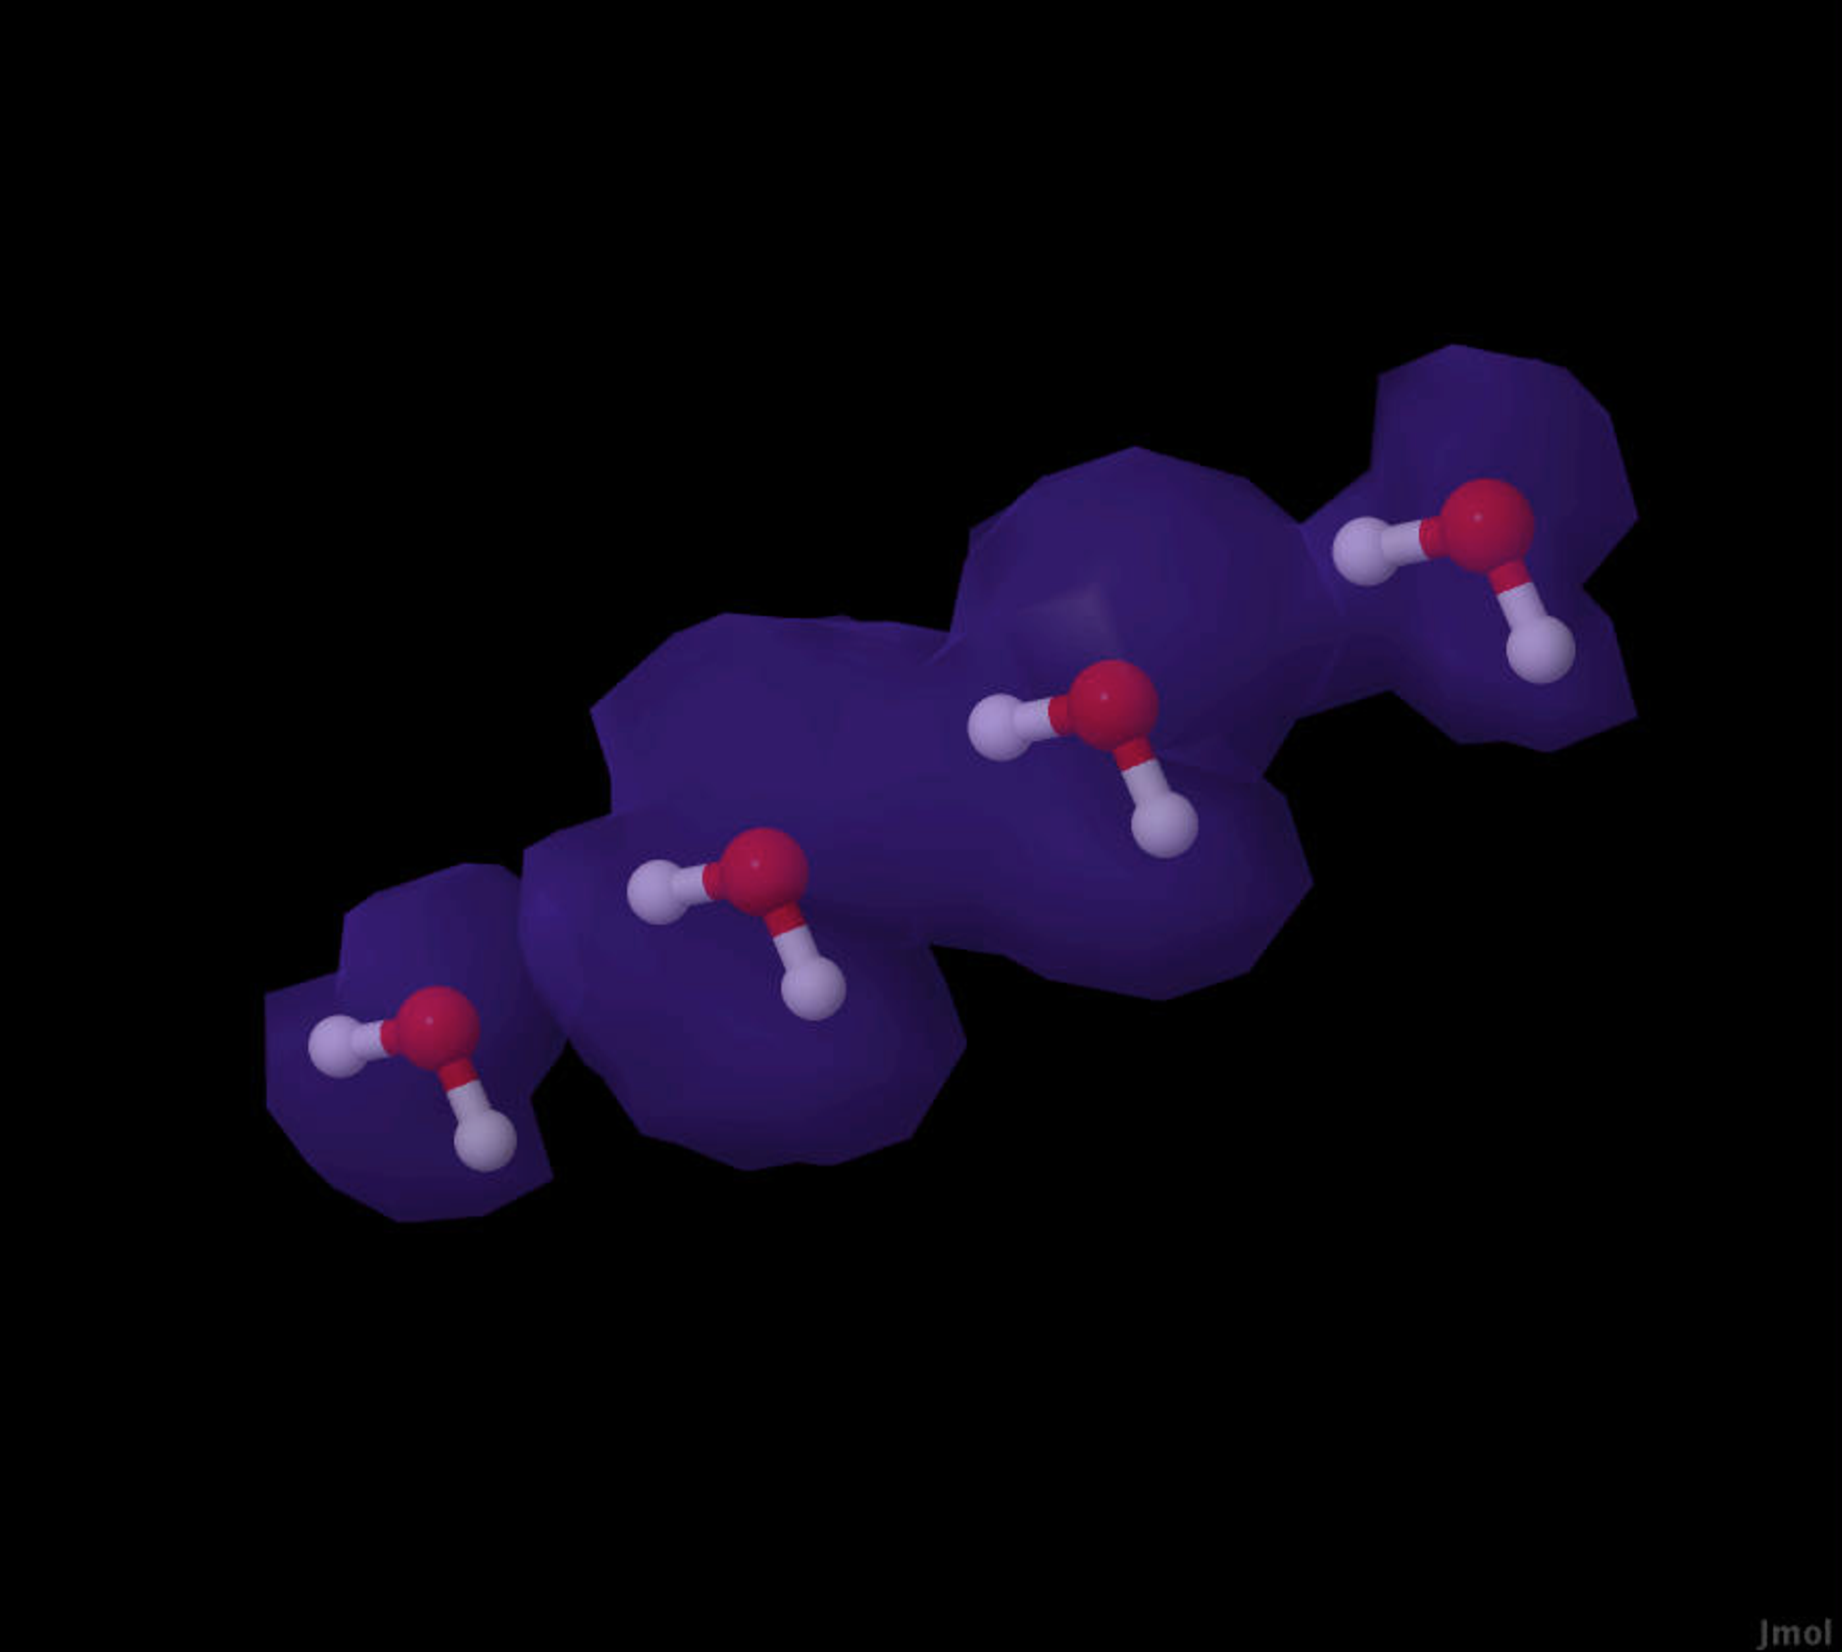
\includegraphics[bb = 60 150 820 670, clip, scale=0.2]{figures/canonical.pdf}
	\end{center}
    \end{column}
    \begin{column}{.48\textwidth}
	\begin{center}
	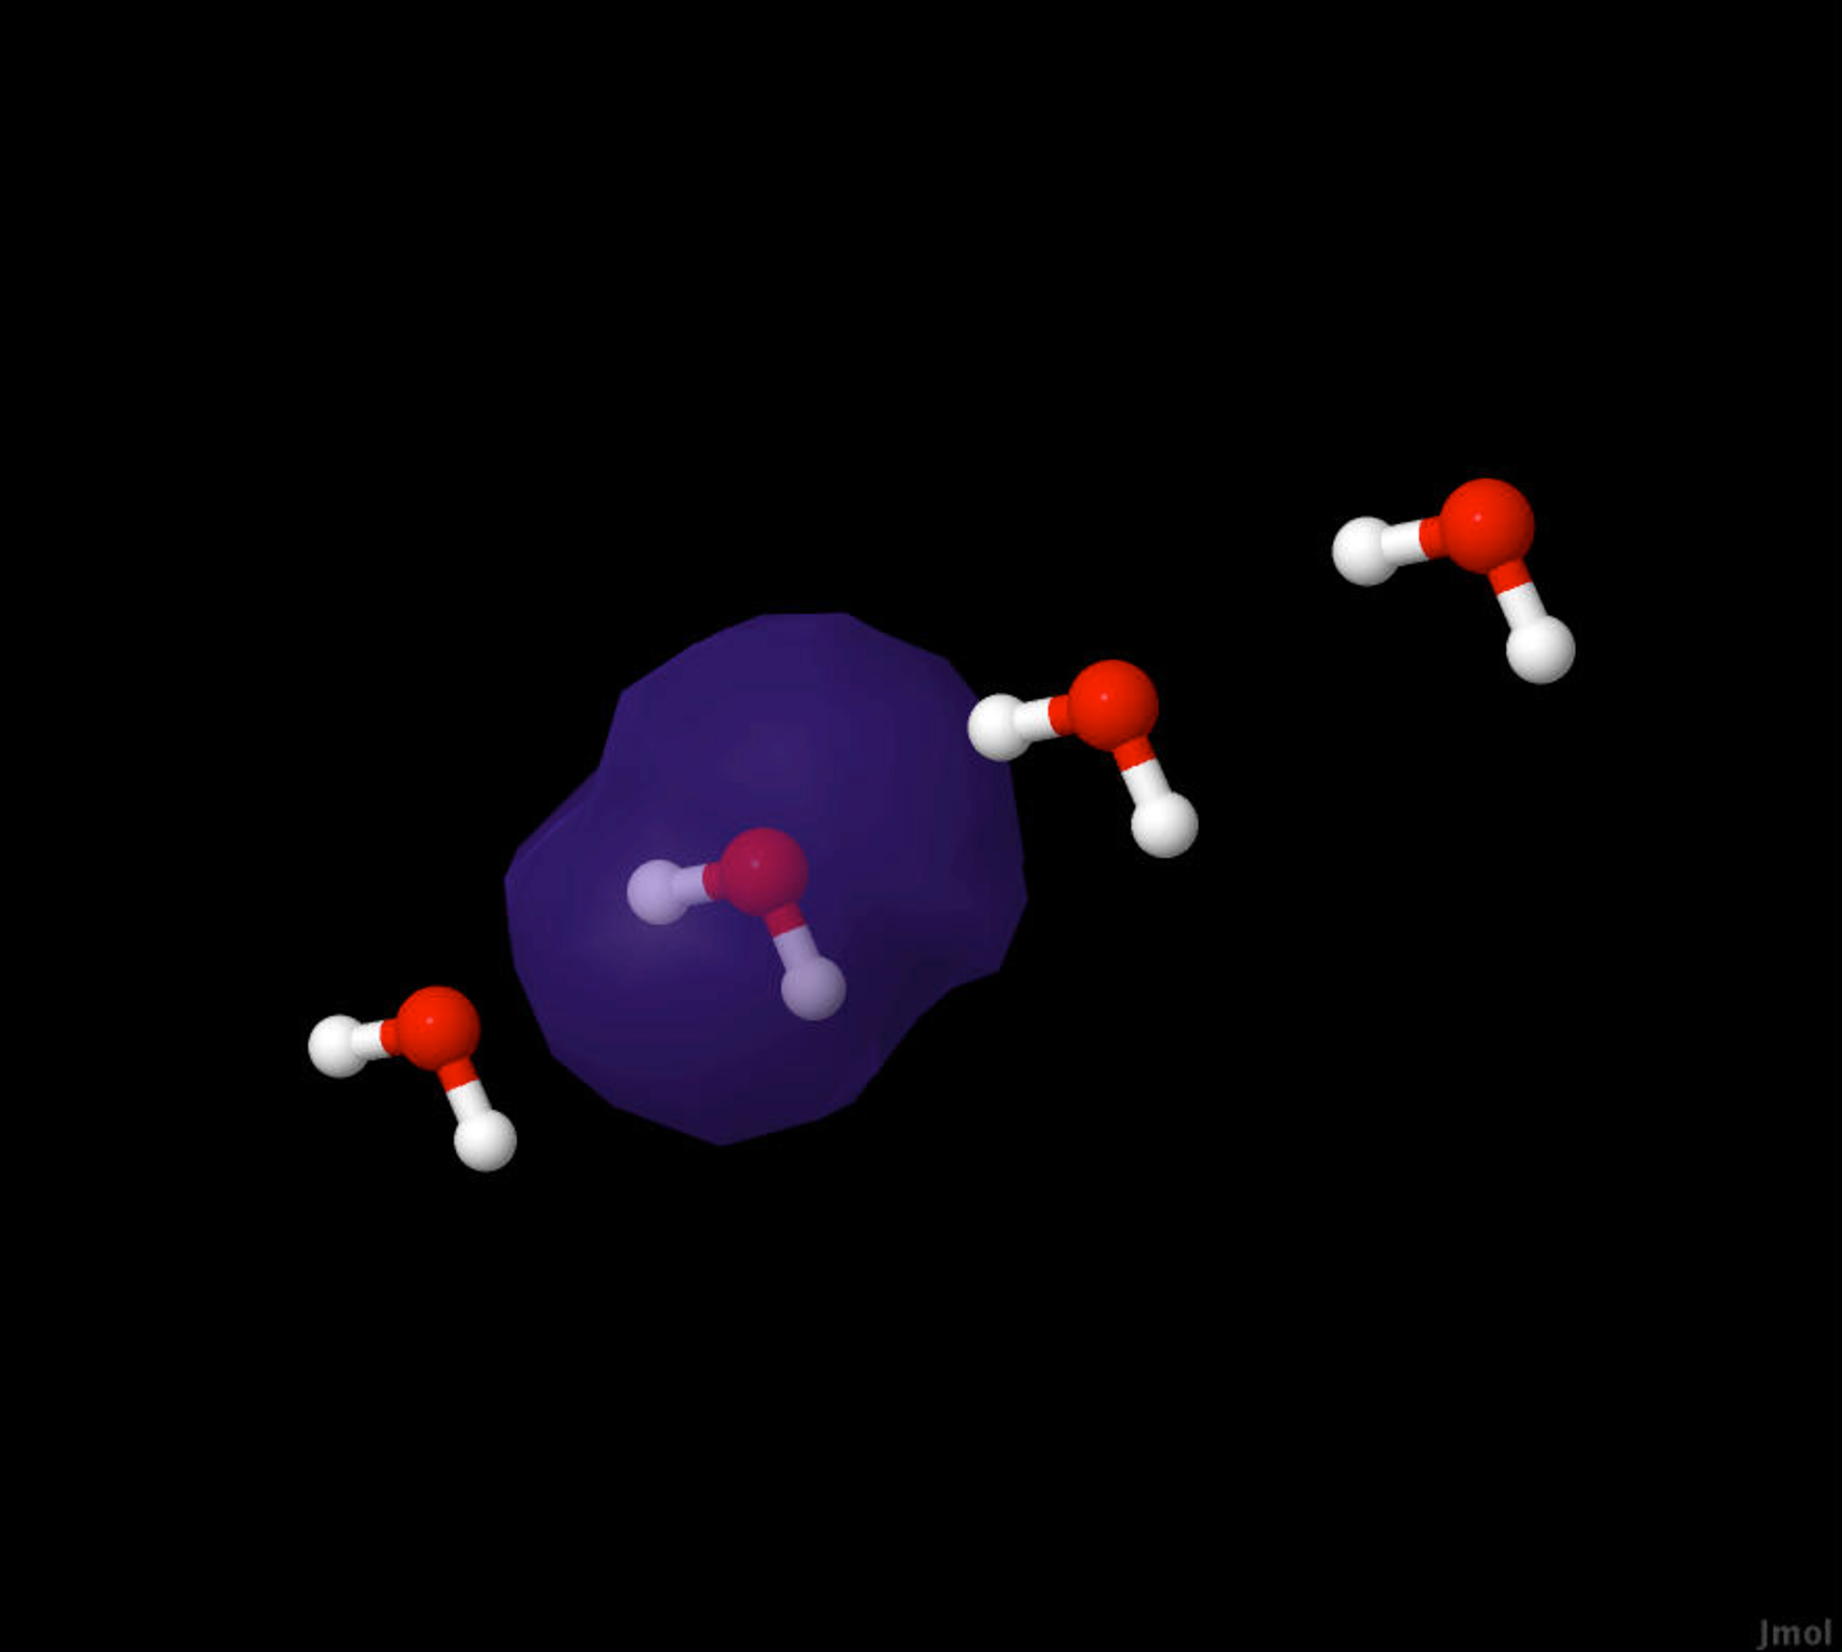
\includegraphics[bb = 60 150 820 670, clip, scale=0.2]{figures/localized.pdf}
	\end{center}
    \end{column}
    \end{columns}
    \ \\
    \ \\
    \tiny \it{J.M.Foster and S.F.Boys; "Canonical Configurational Interaction Procedure" 
	    , Reviews of Modern Physics (1960)}
\end{frame}

\begin{frame}
    \frametitle{Results SCF scaling}
    \begin{center}
    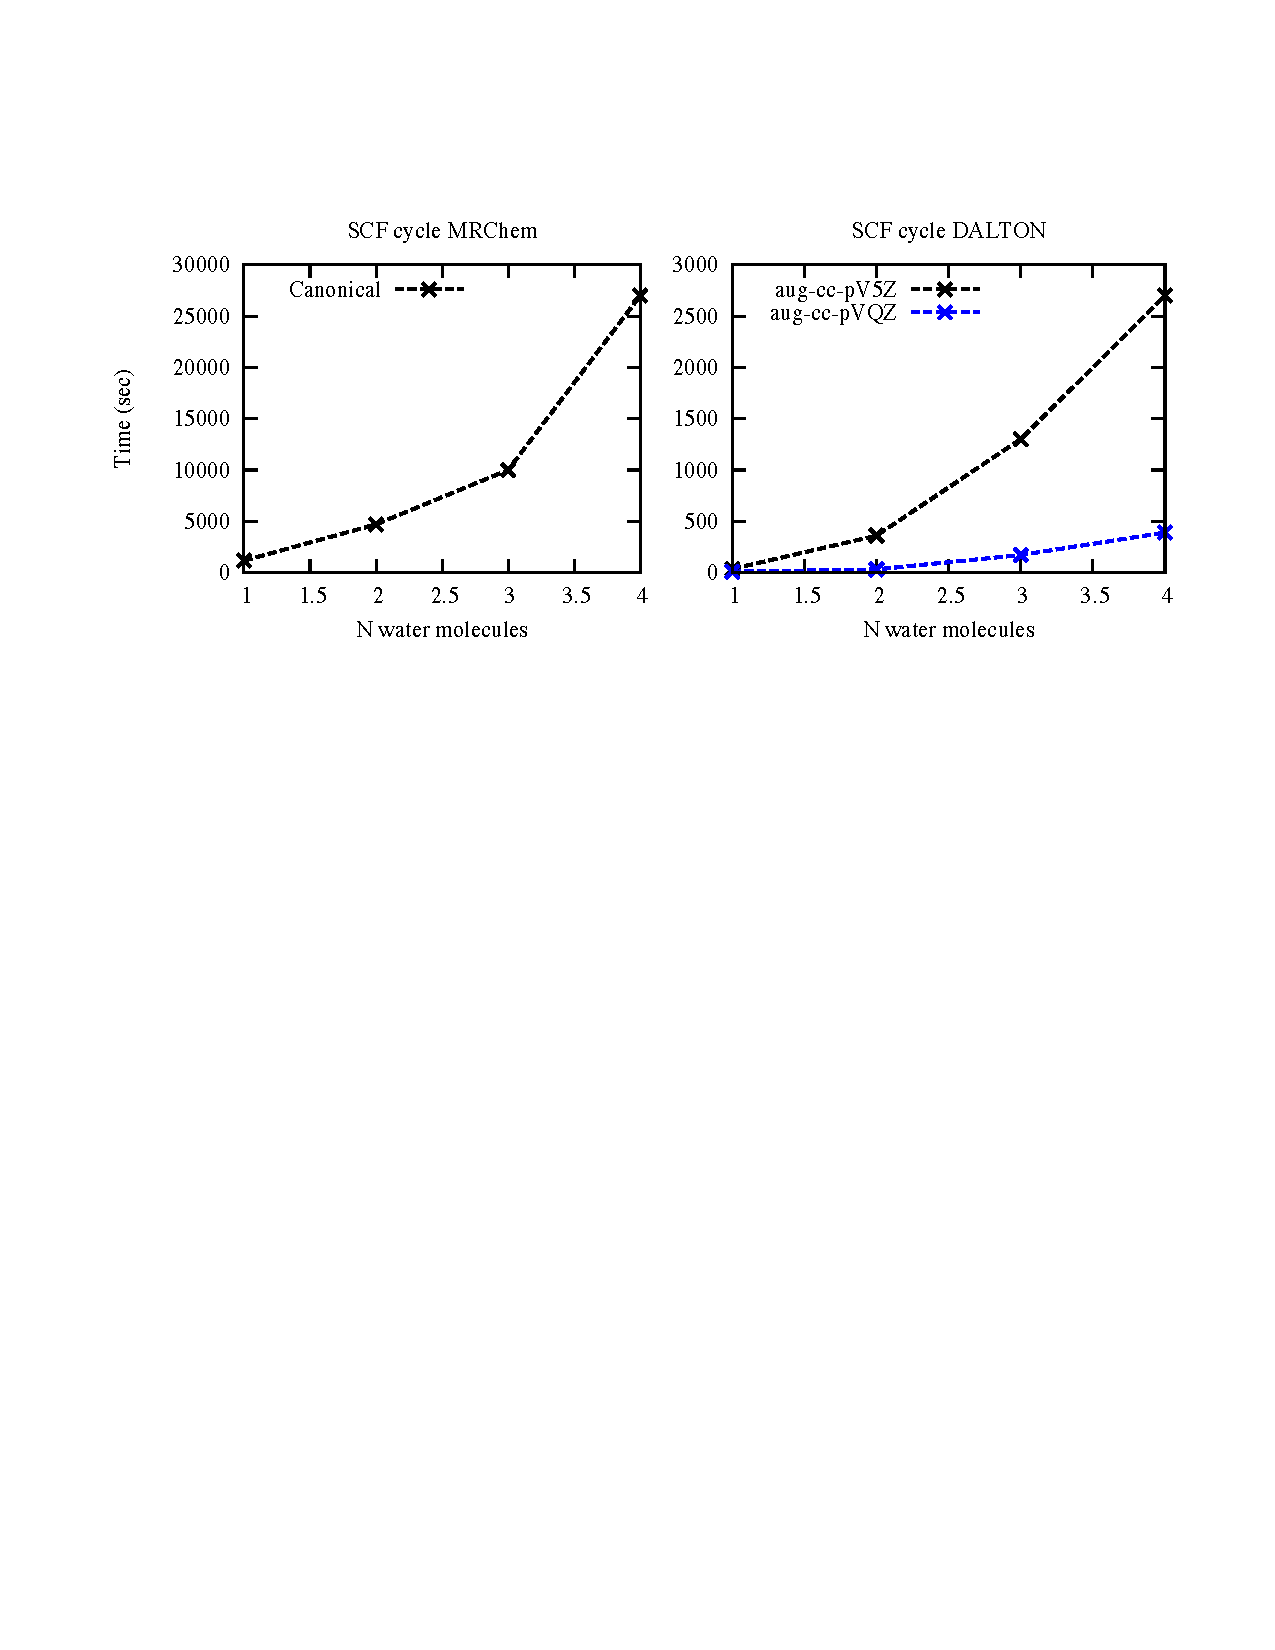
\includegraphics[bb = 50 480 600 700, clip, scale=0.6]{figures/SCFscaling_1.pdf}
    \end{center}
\end{frame}

\begin{frame}
    \frametitle{Results SCF scaling}
    \begin{center}
    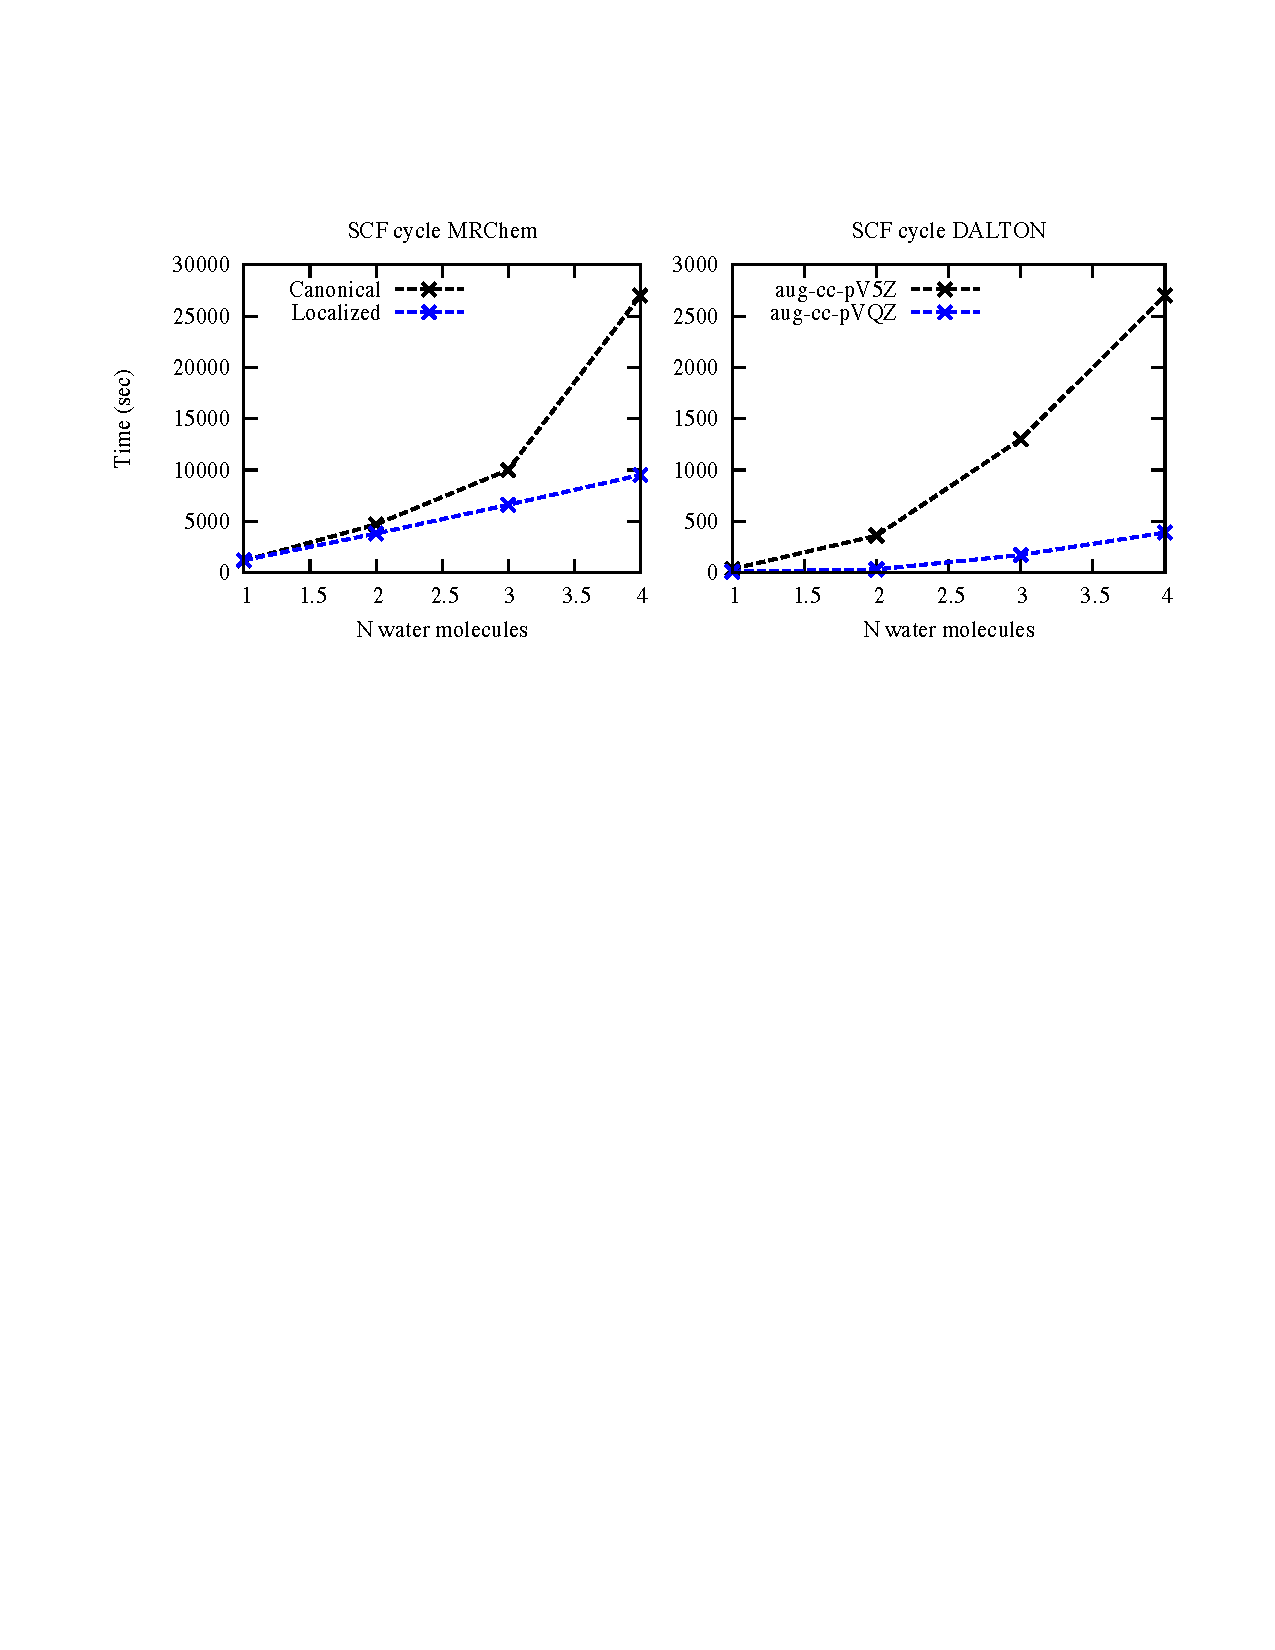
\includegraphics[bb = 50 480 600 700, clip, scale=0.6]{figures/SCFscaling_2.pdf}
    \end{center}
\end{frame}

\begin{frame}
    \frametitle{Results Hartree-Fock}
\begin{table}
\tiny
\begin{tabular}{|c|l|l|l|l|}
\hline Precision     &       H$_2$O &    H$_2$O$_2$ &        HO$_2$ &       O$_2$  \\
\hline MRChem 1.0e-3 & -76.05840640 &  -150.8522985 &  -150.2428723 & -149.7056974 \\
       MRChem 1.0e-5 & -76.06751971 &  -150.8524789 &  -150.2526754 & -149.6915243 \\
       MRChem 1.0e-7 & -76.06753543 &  -150.8524702 &               & -149.6915412 \\
\hline Est. HF limit & -76.0675     &  -150.8525    &  -150.2527    & -149.6915    \\
\hline aug-cc-pCV5Z  & -76.06737937 &  -150.8521878 &  -150.2523966 & -149.6912672 \\
       aug-cc-pCVQZ  & -76.06614045 &  -150.8498523 &  -150.2500956 & -149.6890072 \\
\hline \multicolumn{5}{c}{} \\
       \multicolumn{5}{c}{} \\
\hline Precision     &            C &            CO &        CO$_2$ &   C$_2$H$_2$ \\
\hline MRChem 1.0e-3 & -37.69495687 &  -112.7914472 &  -187.7260422 & -76.85729121 \\
       MRChem 1.0e-5 & -37.69372029 &  -112.7908295 &  -187.7255974 & -76.85533980 \\
       MRChem 1.0e-7 & -37.69374021 &  -112.7908124 &  -187.7253585 & -76.85558532 \\
\hline Est. HF limit & -37.6937     &  -112.7908    &  -187.7254    & -76.8556     \\
\hline aug-cc-pCV5Z  & -37.69369434 &  -112.7906351 &  -187.7250832 & -76.85546957 \\
       aug-cc-pCVQZ  & -37.69338369 &  -112.7891929 &  -187.7226043 & -76.85463825 \\
\hline   \end{tabular} 
\end{table}
    \ \\
    \ \\
    \ \\
    \tiny \it{Michael Harding et.al; "High-accuracy extrapolated ab-initio 
	    thermochemistry", Journal of Chemical Physics (2008)}

\end{frame}

\begin{frame}
    \frametitle{Conclusions}
    We can
    \begin{itemize}
	\item \textcolor{red}{work with localized orbitals}
	\item do \textcolor{red}{low-scaling} Hartree-Fock
	\item do DFT at LDA and GGA level
	\item do both closed- and open-shell systems
	\item obtain basis set limit results for small molecular systems
    \end{itemize}
    \ \\
    \ \\
    \ \\
    \pause
    We cannot
    \begin{itemize}
	\item do post Hartree-Fock methods
	\item compete with traditional Gaussian basis (yet) unless very \\
		high accuracy is required 
    \end{itemize}
\end{frame}

\begin{frame}
    \frametitle{Acknowledgements}
    Chemistry:
    \begin{itemize}
	\item Luca Frediani
    \end{itemize}
    \ \\
    \ \\
    High performance computing:
    \begin{itemize}
    	\item Jonas Juselius
    	\item Peter Wind
    \end{itemize}
    \ \\
    \ \\
    Mathematics:
    \begin{itemize}
	\item Tor Fl\aa
	\item Antoine Durdek
    \end{itemize}
    \ \\
    \ \\
    \ \\
    Contact:
    \begin{itemize}
	\item stig.r.jensen@uit.no
    \end{itemize}
\end{frame}

\end{document}
